\documentclass[11pt,a4paper]{report}
\usepackage[utf8]{inputenc}
\usepackage[left=2cm,right=2cm,top=2cm,bottom=2cm]{geometry}
\usepackage{color}
\definecolor{mygreen}{rgb}{0,0.6,0}
\definecolor{mygray}{rgb}{0.5,0.5,0.5}
\definecolor{mymauve}{rgb}{0.58,0,0.82}

\usepackage{amsthm}
\theoremstyle{definition}
\newtheorem{exinn}{Example}[section]
\newenvironment{example}
{\clubpenalty=10000
	\begin{exinn}%
		\mbox{}%
		{\color{blue}\leaders\hrule height .8ex depth \dimexpr-.8ex+0.8pt\relax\hfill}%
		\mbox{}\linebreak\ignorespaces}
	{\par\kern2ex\hrule\end{exinn}}

\usepackage[english]{babel}
\usepackage{amsmath}
\usepackage{amsfonts}
\usepackage{amssymb}
\usepackage{mathtools}
\usepackage{tocloft}
\usepackage{listings}
\usepackage{graphicx}
\usepackage{tikz}
\usepackage{bigints}
\usepackage{fourier}
\usepackage{fancyhdr}
\pagestyle{fancy}
\usepackage{dsfont}
\usepackage{units}
\usepackage{textcomp}
\usepackage{subcaption}
\usepackage{parskip}
\usepackage{float}
\usepackage{pdfpages}
\renewcommand{\lstlistlistingname}{Code Listings}
\renewcommand{\lstlistingname}{Code Listing}
\definecolor{gray}{gray}{0.5}
\definecolor{green}{rgb}{0,0.5,0}
\lstset{
	tabsize=4,
	rulecolor=,
	language=python,
	%basicstyle=\ttfamily\scriptsize,
	basicstyle=\footnotesize,
	upquote=true,
	numbers=left,
	numberstyle=\footnotesize,
	aboveskip={1.5\baselineskip},
	extendedchars=true,
	linewidth=\linewidth,
	breaklines=false,
	prebreak=\raisebox{0ex}[0ex][0ex]{\ensuremath{\hookleftarrow}},
	frame=single,
	columns=fullflexible,
	showtabs=false,
	showspaces=false,
	showstringspaces=false,
	identifierstyle=\ttfamily,
	keywordstyle=\color[rgb]{0,0,1},
	commentstyle=\color[rgb]{0.133,0.545,0.133},
	stringstyle=\color[rgb]{0.627,0.126,0.941},
}
\pagestyle{fancy}
\lhead{Travis Mitchell}
\rhead{Week 12}
\chead{MECH3750 - Content Summary}
\renewcommand{\headrulewidth}{0.8pt}
\renewcommand{\footrulewidth}{0.8pt}

\author{\textit{Travis Mitchell}}
\title{Lecture Content Summaries for MECH3750}
\date{Updated: 10 October, 2019}			

\makeatletter
\newcommand*{\toccontents}{\@starttoc{toc}}
\makeatother
\renewcommand{\thesection}{\thepart \arabic{section}}


\begin{document}
\section{Treatment of Neumann boundary conditions}
\textit{Simple approach} \\
The simple approach here is to take a one-sided finite difference approximation:
\begin{figure}[!h]
	\centering
	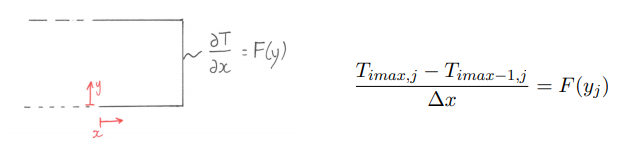
\includegraphics[width=0.8\textwidth]{onesided.png}
\end{figure}
Here, the one-sided difference has been used such that information relies only on the interior of the domain. \\

\textit{Second-order approach}\\
Can you write a second order accurate method for this boundary? What is the form of this and the related error term? \textit{Hint:} can use method of undetermined coefficients, or derive through a Taylor expansion.

\subsection{Symmetry boundary conditions}
This is a special type of Neumann boundary condition in which the derivative with respect to the normal of the domain boundary is 0, 
\begin{align*}
	\frac{\partial T}{\partial \mathbf{n}} = 0.
\end{align*}
Example for Laplace equation:
\begin{figure}[!h]
	\centering
	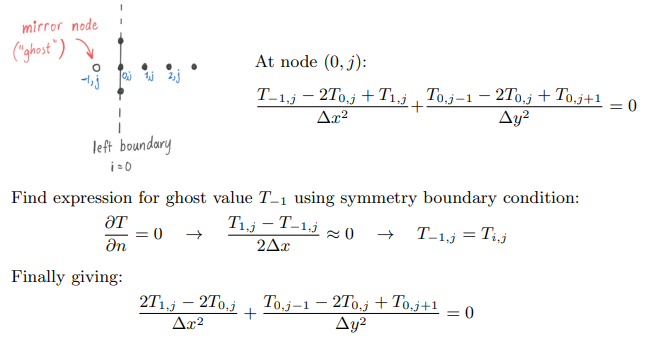
\includegraphics[width=0.8\textwidth]{symmetry.png}
\end{figure}

\section{Discretisation error}
In solving the Laplace (or Poisson) equations, we have been using second order central differences to determine both the second derivative with respect to $x$ and $y$. For some discretisation, $(\delta x, \delta y)$ the corresponding error terms are,
\begin{align*}
	\varepsilon_{xx} &= \frac{\delta x^2}{12}\frac{\partial^4 f}{\partial x^4} (\xi_i,y_j),  \quad \text{with } x_{i-1} \leq \xi_i \leq x_{i+1} \\
	\varepsilon_{yy} &= \frac{\delta y^2}{12}\frac{\partial^4 f}{\partial y^4} (x_i,\eta_j), \quad \text{with } y_{j-1} \leq \eta_i \leq y_{j+1}
\end{align*}
Here it can be seen that the global error is $O(\delta x^2 + \delta y^2)$, namely a second order scheme.

\textit{Boundary influence} \\
What happens when we use a first order one-sided difference for our boundary in this second order scheme? It turns out that `in-general' one can use a boundary discretisation that is one order less than the interior scheme without having a significant impact on the global order of accuracy.

\section{Applying finite difference to real world problems}
\subsection{Verification}
Before we can trust our code, we first have to verify that it is solving what we wanted it to solve. The best way to do this is to compare our error and how this converges in comparison to an analytical solution. Namely, for the Laplace equation we have been looking at, we know our scheme is second order, so with mesh refinement we should approach an analytical solution accordingly.

\subsection{Grid generation}
If only life was lived on a square grid.... To cater for this we can either use an embedded or body-conforming approach,
\begin{figure}[!h]
	\centering
	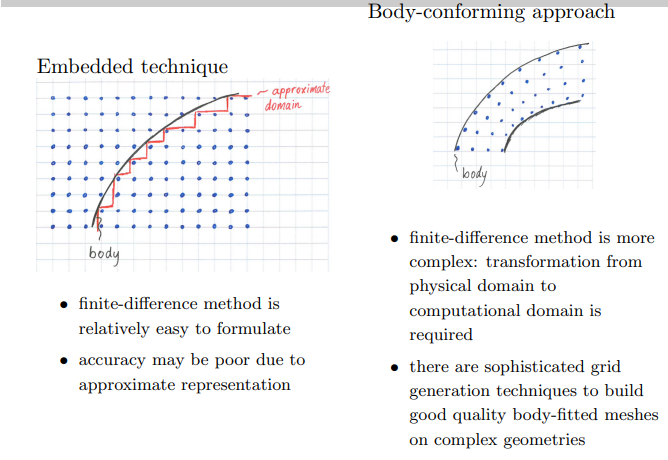
\includegraphics[width=0.8\textwidth]{gridgen.png}
\end{figure}
It turns out that elliptic PDEs can be used for grid generation themselves. So by solving a pre-determined PDE, we can determine the location for our grid points.

\subsubsection{Structured grid generation}
Here we will look at two classes of methods:
\begin{itemize}
	\item algebraic grid generation (e.g. transfinite interpolations) 
	\item PDE-based grid generation (e.g. elliptic grid generation)
\end{itemize}

The use of a PDE solution comes with a number of benefits including the determination of grid locations based solely on the boundary specification and the smoothness of the resulting mesh.


\end{document}
